\documentclass{article}
\usepackage{pgfplots}

\pgfplotsset{compat=1.5.1}

\begin{document}

\makeatletter
\let\tikz@do@circle@orig=\tikz@do@circle

\begin{tikzpicture}
\def\Xmax{3}    \def\Ymax{3}
\def\X{1}       \def\Y{2}
\begin{axis}[
	xmin=-\Xmax,   xmax=\Xmax,
	ymin=-\Ymax,   ymax=\Ymax,
	%
	extra x ticks={-\X,\X},
	extra y ticks={-\Y,\Y},
	extra tick style={grid=major},
]
	\draw[black] (axis cs:0,0)
		ellipse [          x radius=10pt,y radius=20pt];
	\draw[black] (axis cs:0,0)
		ellipse [          x radius=\X,y radius=\Y];
	\draw[red]   (axis cs:0,0)
		ellipse [rotate=90,x radius=\X,y radius=\Y];
	\draw[green]   (axis cs:0,0)
		circle [radius=1];
	\addplot [only marks,mark=*] coordinates { (0,0) };

	\node at (axis cs:-2,-2) {
		\ifx\tikz@do@circle\tikz@do@circle@orig
		\else
			\PackageError{pgfplots}{ASSERTION FAILED: tikz@do@circle is wrong}{}
		\fi
		\tikz \draw[x={(1cm,0cm)},y={(0cm,1cm)}] 
			ellipse[x radius=1,y radius=1];
	};
\end{axis}
\end{tikzpicture}

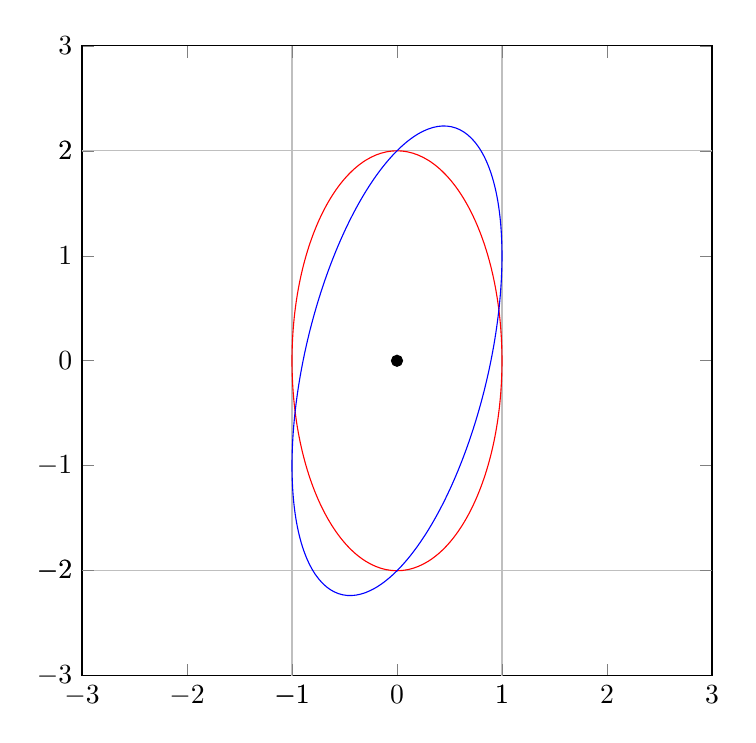
\begin{tikzpicture}
\def\Xmax{3}    \def\Ymax{3}
\def\X{1}       \def\Y{2}
\begin{axis}[
	width=8cm,  height=8cm,
	scale only axis=true,
	%
	xmin=-\Xmax,   xmax=\Xmax,
	ymin=-\Ymax,   ymax=\Ymax,
	%
	extra x ticks={-\X,\X},
	extra y ticks={-\Y,\Y},
	extra tick style={grid=major},
]
	\draw[red]
		\pgfextra{
			\pgfpathellipse{\pgfplotspointaxisxy00}
				{\pgfplotspointaxisdirectionxy{\X}{0}}
				{\pgfplotspointaxisdirectionxy{0}{\Y}}
		};
	\draw[blue]
		\pgfextra{
			\pgfpathellipse{\pgfplotspointaxisxy00}
				{\pgfplotspointaxisdirectionxy{1}{1}}
				{\pgfplotspointaxisdirectionxy{0}{2}}
		};
	\addplot [only marks,mark=*] coordinates { (0,0) };
\end{axis}
\end{tikzpicture}
\end{document}
